% Reports (up to ~2500 words including references, notes and captions–corresponds to ~3 printed pages in the journal) present important new research results of broad significance. Reports should include an abstract, an introductory paragraph, up to four figures or tables, and about 30 references. Materials and Methods should be included in supplementary materials, which should also include information needed to support the paper's conclusions.

% Main Text is not divided into sub-headings for Reports. 

% The manuscript should start with a brief introduction describing the paper’s significance. The introduction should provide sufficient background information to make the article intelligible to readers in other disciplines, and sufficient context that the significance of the experimental findings is clear. 

% \clearpage

Since early 2020, the CoViD-19 pandemic has presented an enormous challenge to humanity
on many dimensions. The development of highly effective vaccines holds the promise of
containment in the medium term. However, most countries find themselves many months---and
often years---away from reaching vaccination-induced herd immunity.\comment[id=HM]{Cite
some paper on herd immunity, maybe vaccine data} In the meantime, it is of utmost
importance to employ an effective mix of strategies for containing the virus. The most
frequent initial response was a set of non-pharmaceutical interventions (NPIs) to reduce
contacts between individuals. While this has allowed some countries to sustain equilibria
with very low infection numbers\footnote{See \citet{Contreras2021} for a theoretical
equilibrium at low case numbers which is sustained with test-trace-and-isolate
policies.}, most have seen large ups and downs in their infection rates. Containment
measures have become increasingly diverse and included testing, more nuanced NPIs, and
contact tracing. Neither these policies' effect nor the influence of seasonal patterns or
more infectious virus strains are well understood in quantitative terms. This paper
develops a model incorporating all these factors. The framework allows to combine a wide
variety of data in a timely fashion, making it useful to predict the effects of various
interventions. We apply the model to Germany and show that rapid testing had the largest
impact on the reduction in infections by XXX\% during the A weeks between X April and Y
May.\comment[id=HM]{insert some useful numbers}. We conclude that rapid tests should play
a large role...

At the core of our agent-based model are physical contacts between heterogeneous agents
(Figure~\ref{fig:broad_model_description}).\footnote{We provide a detailed comparison to
other approaches in \ref{sec:literature_review}. The model most closely related to ours
is described in \citet{Hinch2020}.} Each contact between an infectious individual and
somebody susceptible to the disease bears the risk of transmitting the virus. Contacts
occur in the household, at work, at school, or in other settings (leisure activities,
grocery shopping, medical appointments, etc.).\comment[id=HM]{Systemic relevance of
work?} Some contacts recur regularly, others occur at random. Random contacts are
typically assortative in age and geographical location. Empirical applications can take
the population structure from census data and the types and frequency of contacts from
diary data measuring contacts before the pandemic
\citep[e.g.][]{Mossong2008}.\footnote{\citet{Hoang2019} provide access to multiple data
sets on contact types and frequencies at \url{http://www.socialcontactdata.org/} covering
countries from all continents except North America and Australia.} The dimensions are
chosen so that the most common NPIs can be modeled in great detail by reducing the number
of contacts in a particular setting or the risk of transmitting the disease for a type of
contact. For example, a mandate to work from home will reduce the number of work contacts
to zero for a fraction of the working population. Schools and daycare can be closed
entirely, operate at reduced capacity including an alternating schedule, or implement
mitigation measures like masking requirements or air filters \citep{Lessler2021}. Curfews
may reduce the number of contacts in non-work/non-school settings. In any setting,
measures like masking requirements would reduce the probability of infection associated
with a contact.

\begin{figure}[!tp]
    \centering

    \begin{subfigure}[b]{0.425\textwidth}
        \centering
        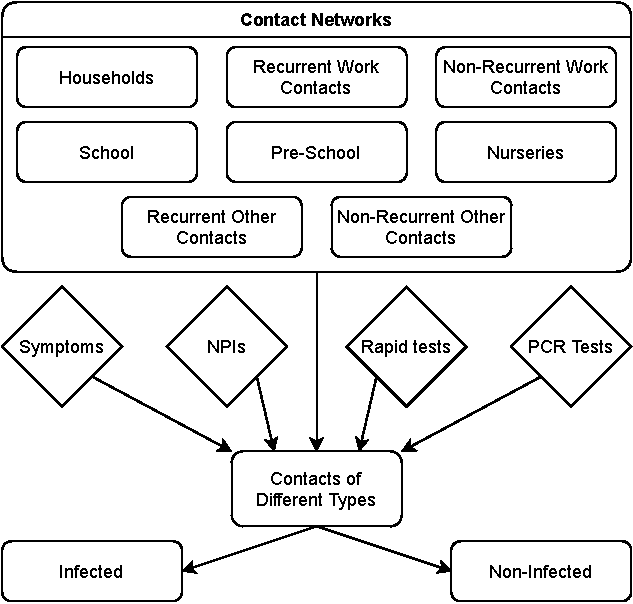
\includegraphics[width=\textwidth]{../figures/model-graph-top-left}
        \caption{{\small Model description}}
        \label{fig:broad_model_description}
    \end{subfigure}
    \hfill
    \begin{subfigure}[b]{0.425\textwidth}
        \centering
        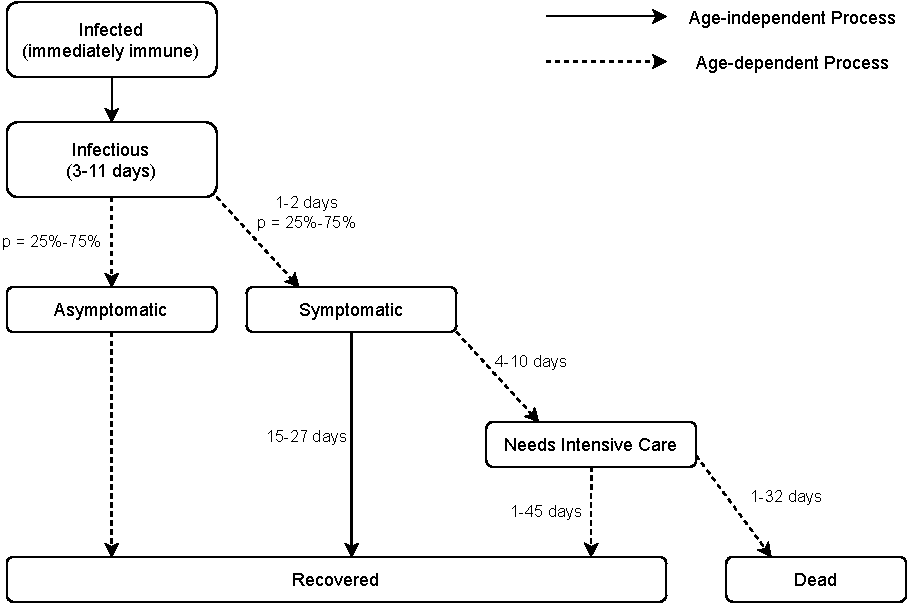
\includegraphics[width=\textwidth]{../figures/model-graph-top-right}
        \caption{Disease progression}
        \label{fig:disease_progression}
    \end{subfigure}
    \vskip3ex
    \begin{subfigure}[b]{0.425\textwidth}
        \centering

        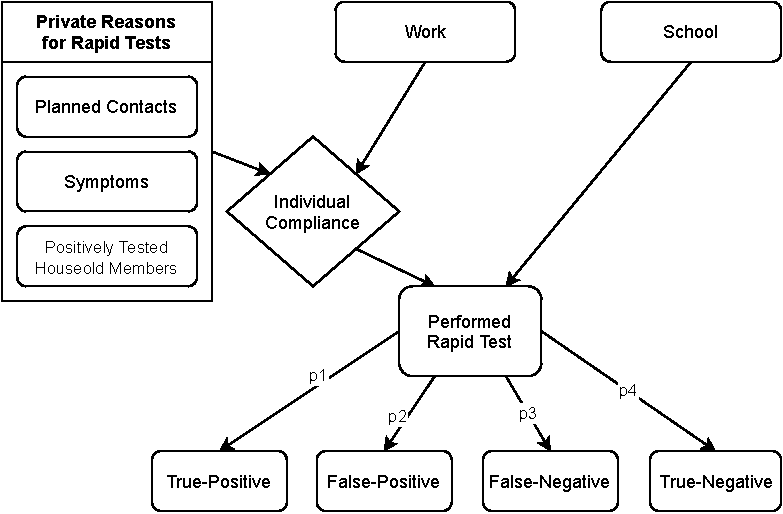
\includegraphics[width=\textwidth]{../figures/model-graph-bottom-left}
        \caption{{\small PCR and antigen tests}}
        \label{fig:pcr_antigen_tests}
    \end{subfigure}
    \hfill
    \begin{subfigure}[b]{0.425\textwidth}
        \centering

        Model for detected/undetected cases

        % 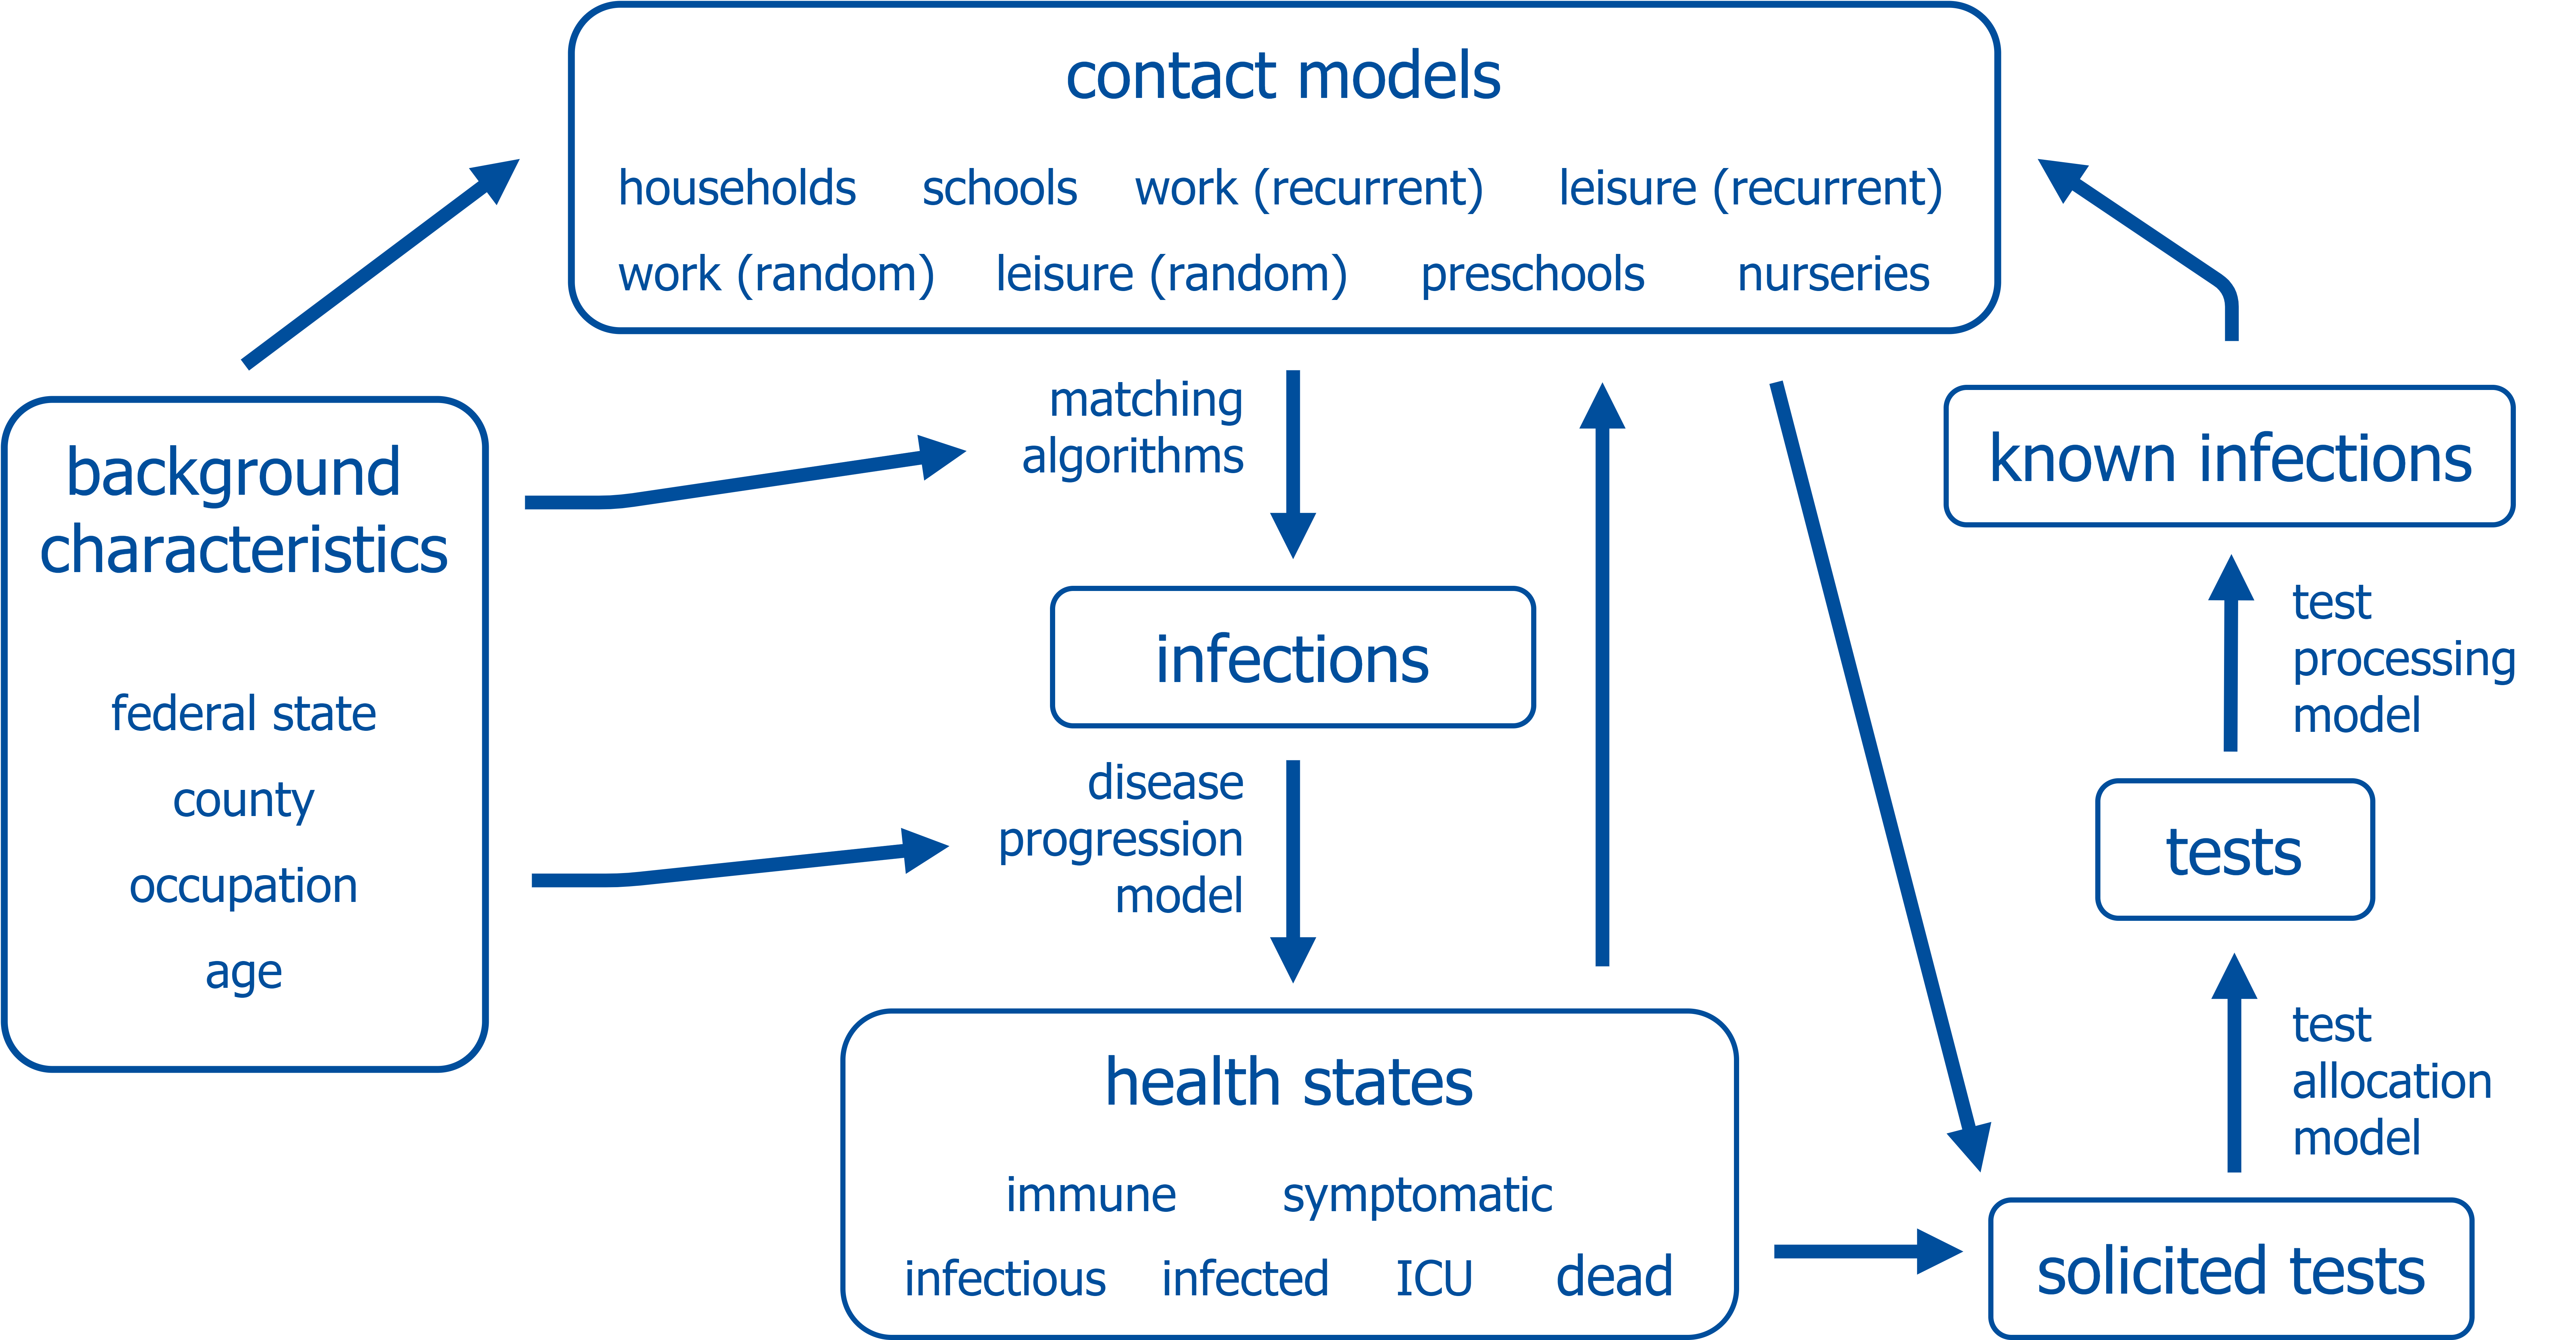
\includegraphics[width=\textwidth]{../figures/model_detailed.png}
        \caption{{\small Model for translating simulated number to officially recorded cases}}
        \label{fig:model_for_official_cases}
    \end{subfigure}

    \caption{Model description}
    \label{fig:model-description}

    \floatfoot{\noindent
        Note: ...
    }

\end{figure}

Susceptibility to contracting the SARS-CoV-2 virus is dependent on age; so is the
progression of a possible infection. We differentiate between an initial period of
infection without being infectious or showing symptoms, being infectious (presymptomatic
or asymptomatic), showing symptoms, requiring intensive care, and recovery or death. The
probabilities of transitioning between these states depend on age; their duration is
random within intervals calibrated to medical literature (for a detailed description see
Section~\ref{sec:medical_params}).
Conditional on the type of contact, infectiousness independent of ages \citep{Jones2021}.

The model includes several other features, which are crucial to describe the evolution of
the pandemic in 2020-2021. New virus strains with different profiles regarding
infectiousness and disease progress can be introduced. With a probability calibrated to
\cite{Hunter2021}, vaccinated agents become immune and they do not
transmit the virus \citep{Petter2021, LevineTiefenbrun2021, Pritchard2021}.
% the sources only report reduced viral shedding and reduced risk of infection.
% Lauterbach calculated that taking the risk of infection * reduced infectiousness given
% infection based on theses studies suggest that given exposure the risk that fully
% vaccinated individuals pose is <10% of an unvaccinated person.
While vaccines are rolled out, priority may depend on age and occupation. Agents may
demand two types of tests as described in Figure~\ref{fig:pcr_antigen_tests}. First,
polymerase chain reaction (PCR) tests directly reveal whether an individual is infected
or not. PCR tests require some time to be processed and there are always aggregate
capacity constraints. Second, rapid antigen tests yield immediate results. Specificity
and sensitivity of these tests is set according to data by \cite{Bruemmer2021, Smith2021}
. The sensitivity of the rapid antigen tests depends on the timing of the test relative
to the start of infectiousness.\comment[id=HM]{subsequent PCR tests, quarantine,
work/school}. Demand for rapid tests will depend on policy, e.g., prices, testing
requirements before work, attending school, or visiting restaurants and shops.

Modelling a population of agents according to actual demographic characteristics means
that we can use a wide array of data to identify and estimate the model's many
parameters.\footnote{See section S.X of the supplementary materials for an
overview.}\comment[id=HM]{Need to make a list including symbols, maybe you can fetch the
parameters from the model and then we brainstorm re notation?} Mobility data is used to
model the reductions in work contacts. School and daycare policies are incorporated
directly from official directives. Infection rates by age and geographical region are
estimated to match to officially recorded numbers; so is the prevalence of virus strains.
In order to translate simulated cases in our model to officially recorded cases, we use
the model depicted in Figure~\ref{fig:model_for_official_cases}. \comment[id=HM]{Add a
sentence.} A further advantage is that the simulated data have a structure that resembles
datasets used for regression models, which allows additional plausibility checks by
re-running the same models on the model-generated data.\comment[id=HM]{Only keep if we
actually do something like that.}

Model that makes the most of many available data sources to gauge the relative effects in
this transition period -- see joint distribution of infections with age, geography. But
contacts with age, geography, occupations.

We apply this model to Germany. In March and April 2020, the country broke the first wave
of the pandemic fairly quickly. Between mid-May and mid-September, daily new infections
were below 20 per Million and day.\comment[id=HM]{Cite our world in data} We model the
period mid-September 2020 to the end of May 2020. We pick the starting date for two
reasons. First, we do not include the first wave because the environment was very
different (e.g., aggregate PCR test capacity was much lower and we would require a very
different model for calculating the share of known cases) and some data was not recorded
yet.\comment[id=HM]{True?}\comment[id=K]{We would definitely need to model national
and international travel which you mention below. Regarding data I think everything would
be available. The low numbers during summer in our sample size might also be a problem
because Covid might go extinct in our model when case numbers are so low.}. Second, a
large fraction cases during summer of 2020 were traced to international
travel,\comment[id=HM]{cite \url{https://www.rki.de/DE/Content/Infekt/EpidBull/Archiv/2021/Ausgaben/08_21.pdf}}, but the precise number is difficult to model.

Figure~\ref{fig:pandemic_drivers_model_fit} describes the evolution of the pandemic and
of its drivers. The black line in Figure~\ref{fig:aggregated_fit} shows officially
recorded cases; the \replaced[id=HM]{color}{blue?} line in
Figure~\ref{fig:stringency_index} the Oxford Response Stringency Index \citep{Hale2020},
which tracks the tightness of non-pharmaceutical interventions. We transform the index so
that lower values represent higher levels of restrictions. A value of zero means all
measures incorporated in the index are turned on. The value 1 represents the situation of
mid-September, where half of all restrictions incorporated in the index are
active.\comment[id=HM]{Need to find version of index with a couple of measures, probably
need the API access...}. In the six weeks between mid September and mid October, cases
increased by a factor of 3.\comment[id=Klara]{In the next iteration all empirical data is
in the figures/results/tables/empirical_analogues.csv}
% the week of Sep 13 had an incidence of 12.4, the week of Oct 18 had 51.
Restrictions were somewhat tightened in mid-October and again in early November. New
infections remained constant throughout November, before rising again in December.

\begin{figure}[!tp]
    \centering

    \begin{subfigure}[b]{0.475\textwidth}
        \centering
        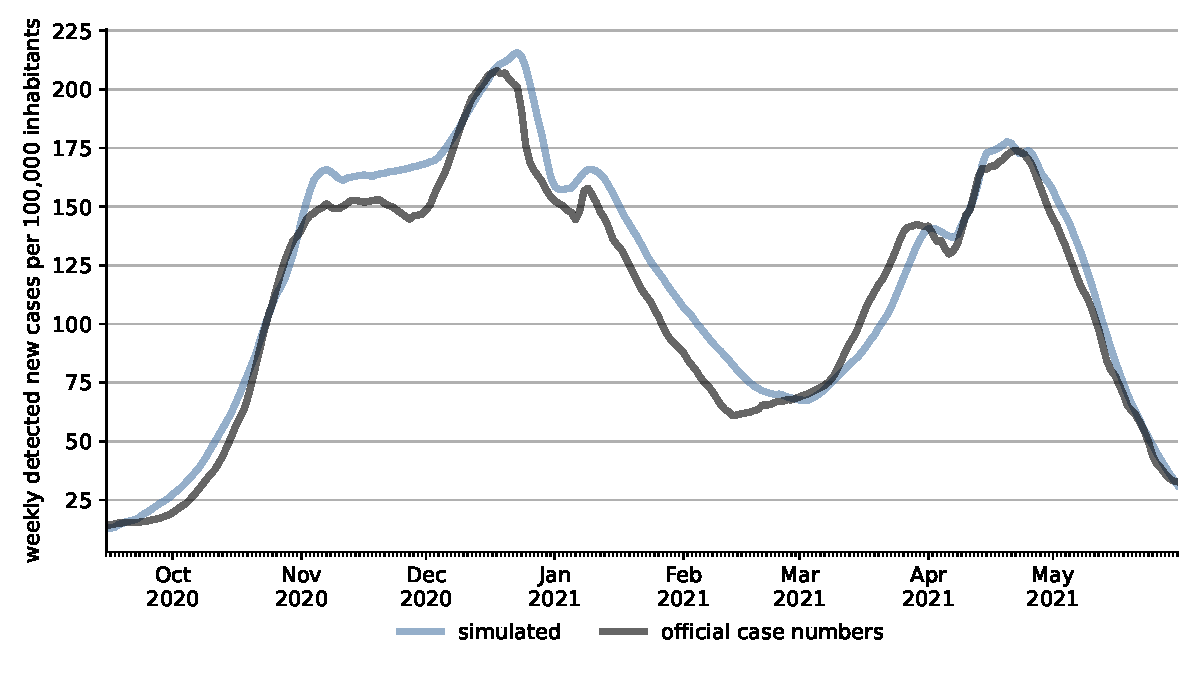
\includegraphics[width=\textwidth]{../figures/results/figures/scenario_comparisons/combined_fit/full_new_known_case}
        \caption{{\small Recorded cases: Empirical and simulated}}
        \label{fig:aggregated_fit}
    \end{subfigure}
    \hfill
    \begin{subfigure}[b]{0.475\textwidth}
        \centering
        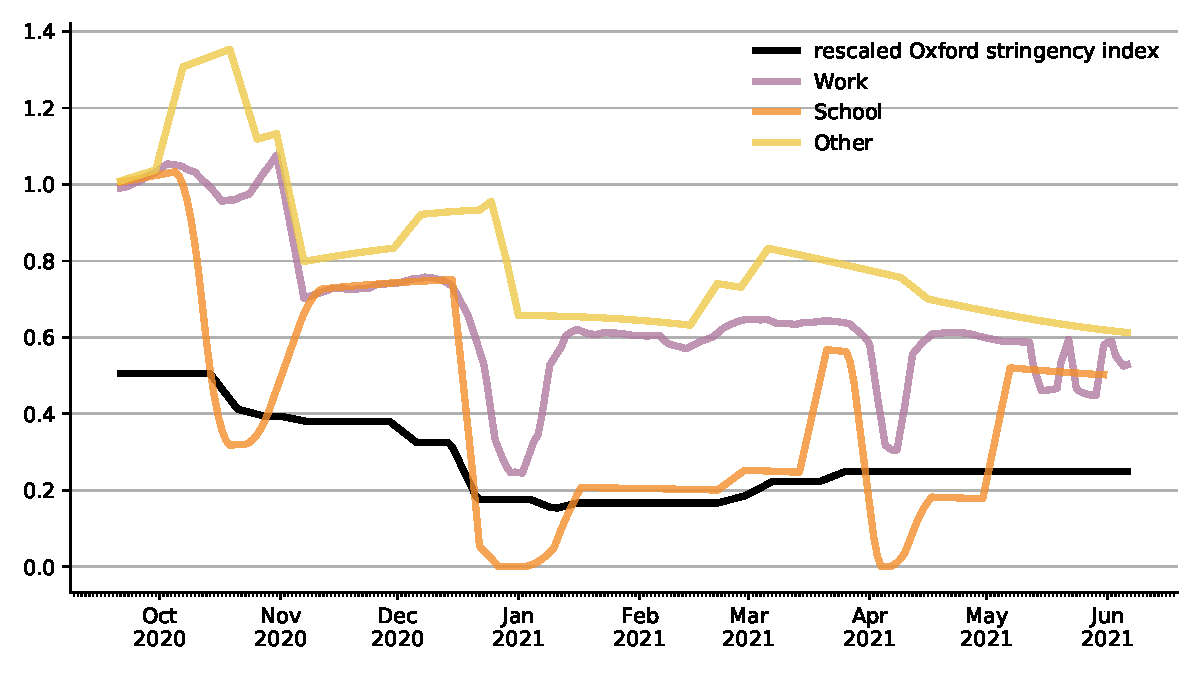
\includegraphics[width=\textwidth]{../figures/results/figures/data/stringency_with_seasonality}

        \caption{{\small Stringency of NPIs and changes in infectious contacts by type}}
        \label{fig:stringency_index}
    \end{subfigure}

    \vskip3ex

    \begin{subfigure}[b]{0.475\textwidth}
        \centering

        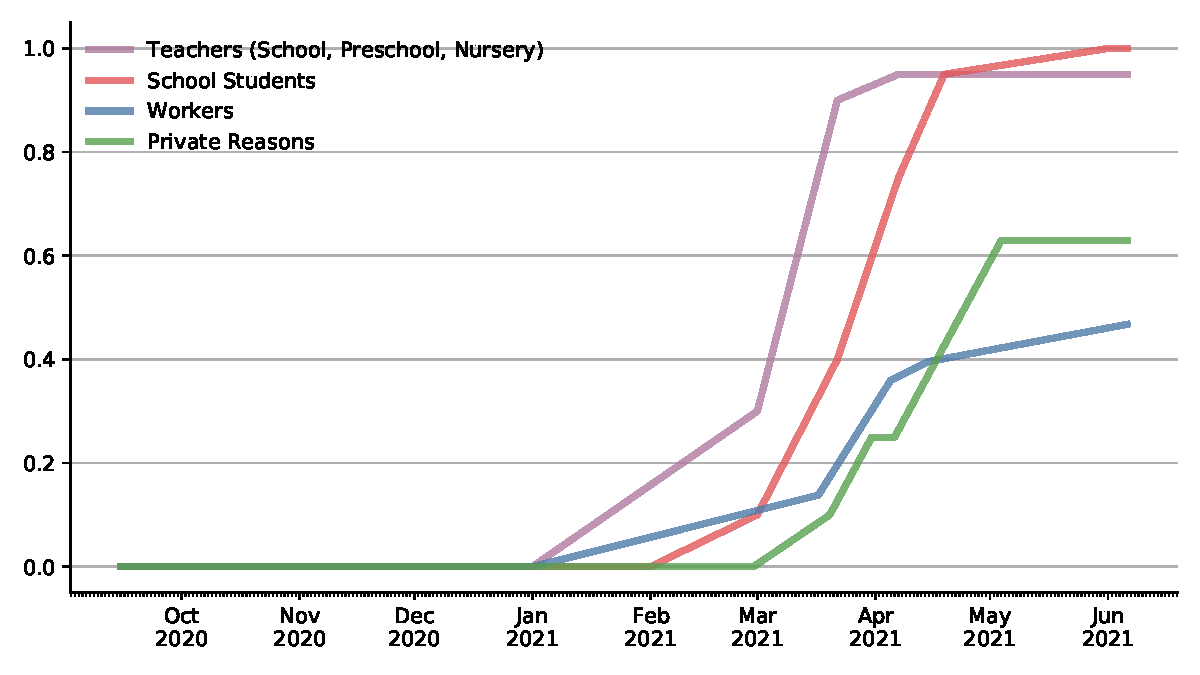
\includegraphics[width=\textwidth]{../figures/results/figures/data/testing/rapid_test_demand_shares}

        \caption{{\small Tests and vaccinations}}
        \label{fig:antigen_tests_vaccinations}
    \end{subfigure}
    \hfill
    \begin{subfigure}[b]{0.475\textwidth}
        \centering
        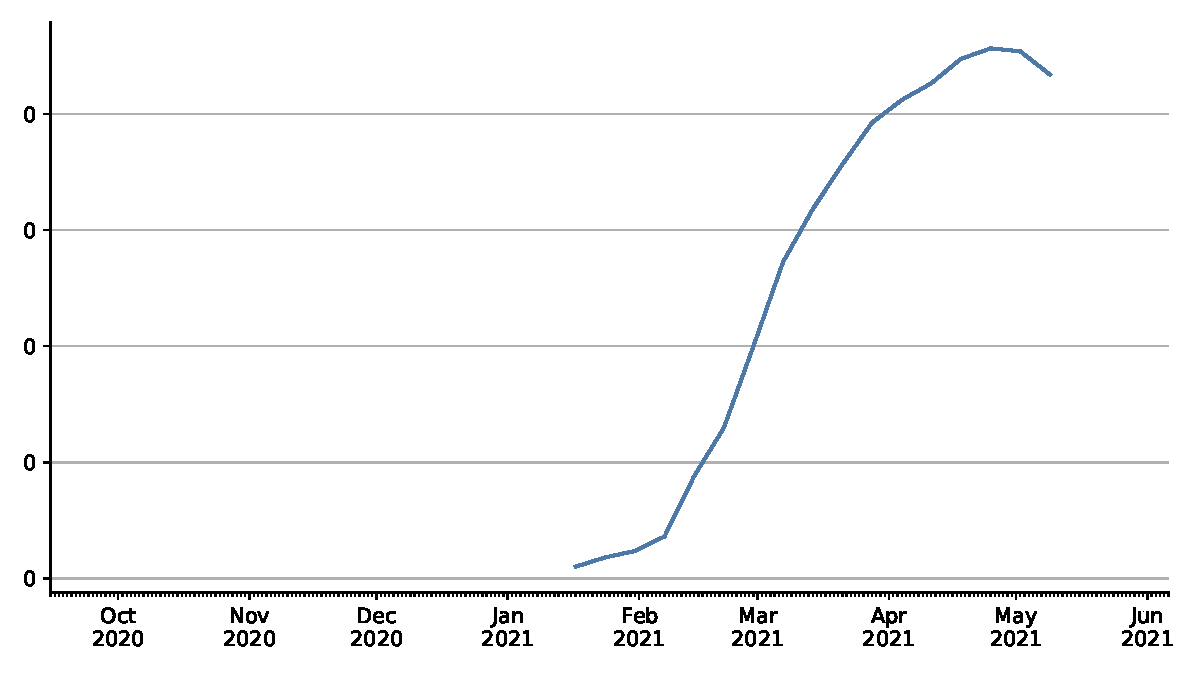
\includegraphics[width=\textwidth]{../figures/results/figures/data/share_of_b117_acc_to_rki}

        \caption{Fraction of B.1.1.7 strain among measured infections}

        \textcolor{red}{We'll have this compared to our baseline simulation in the next
        iteration.}
        \label{fig:share_b117}
    \end{subfigure}

    \caption{Evolution of the pandemic, its drivers, and model fit, September 2020 to May 2021}
    \label{fig:pandemic_drivers_model_fit}

    \floatfoot{\noindent
        Note: All aggregates; See S.XXX for statistics by age group and by geographical region. Also more disaggregated data.

        Sources: ...
    }

\end{figure}

Quickly rising rates in December prompted the most stringent lockdown to this date. Schools and daycare centers were closed again, so were customer-facing businesses except for grocery and drug stores. Shortly afterwards, more factors become relevant. Just after Christmas, the first people were vaccinated with a focus on older age groups and medical personnel (Figure~\ref{fig:antigen_tests_vaccinations}. By the end of May, just over 40\% had received at least one dose of a vaccine. Starting in January, rapid tests \dots These had to be administered by medical doctors or in pharmacies. At-home tests approved by authorities were ... in March.\comment[id=HM]{update precise timeline}\comment[id=Klara]{From a docstring:Bürgertests started in mid March but demand was very low initially (\url{https://bit.ly/3ehmGcj}). First tests to self-administer became available starting March 6. However, supply was very limited in the beginning (\url{https://bit.ly/3xJCIn8}).} From the peak of the second wave just before Christmas until the trough in mid-February, newly detected cases decreased by almost three quarters. The third wave in the spring of 2021 is associated with a rise in the share of the B.1.1.7 variant among all infections, depicted in Figure~\ref{fig:share_b117}, reaching more than 80\% in April\comment[id=HM]{Do we have the table somewhere?}\comment[id=Klara]{Will be part of the empirical analogues table}. In early March, some NPIs were being relaxed; e.g., hairdressers and home improvement stores were allowed to open again to the public. In some cases, customers were only allowed to enter with a recent negative rapid test result.

These developments are characteristic of many countries: The initial focus on NPIs to slow the spread of the disease has been accompanied by vaccines and a growing acceptance and use of rapid tests. At broadly similar points in time, novel strains of the virus have started to pose additional challenges. The blue line in Figure~\ref{fig:aggregated_fit} shows that our model tracks the simulated infections extremely well. This is also true for infections by age and geographical region, which are shown in the supplementary materials (figures~\ref{fig:age_group_fit, fig:state_fit}. We can disentangle various mechanisms due to the distinct temporal variation in the drivers of the pandemic. Next to the stringency index, the three lines in Figure~\ref{fig:stringency_index} summarize how contact reductions, increased hygiene regulations, and seasonality evolved since early September for each of the three broad contact networks. For example, a value of 0.75 for the work multiplier means that if the environment was the same as in September (levels of infection rates, no rapid tests or vaccinations, only the wildtype virus present), infections at the workplace would be reduced by 25\%. This reduction is the product of the effect of contact reductions, increased hygiene regulations, and seasonality. Along with the levels of infections, these measures completely determine the spread of SARS-CoV-2 in 2020.\comment[id=HM]{True?} See Appendix~\comment[id=HM]{Reference} for their individual contributions. Two things are particularly interesting. First, all lines broadly follow the stringency index and they would do so even more if we left out seasonality. Second, the most stringent regulations are associated with the period of strong decreases in new infection beteen late December 2020 and mid-February 2021. The measures were not enough, however, to stop the B.1.1.7 variant from spreading in the subsequent period. The steep drop in recorded cases during May 2021 is associated with rapid tests to X-Y~percent of the population, a vaccination rate that rose from 25\% to 4X\%, and mostly seasonality impacting a fall in the relative infectiousness of contacts outside of work and school\comment[id=HM]{check with corrected graph}.

Figure~\ref{fig:2021_scenarios_broad} consider the relative effects of rapid tests, vaccinations, and of seasonality during 2021, assuming NPIs to have evolved the same way as in the baseline scenario. Figure~\ref{fig:2021_scenarios_recorded} shows the model fit (the bold blue line\comment[id=HM]{Make sure this is the case}, same as in Figure~\ref{fig:aggregated_fit}), a scenario without any of the three factors (x line), and three scenarios turning these factors off one by one. Figure~\ref{fig:2021_scenarios_newly_infected} does the same for total infections in the model. Figure~\ref{fig:2021_scenarios_decomposition} employs Shapley values to decompose the difference in total infections between the scenario without any of the three factors and our main specification.

\begin{figure}[!tp]
    \centering
    
    \begin{subfigure}[b]{0.475\textwidth}
        \centering
        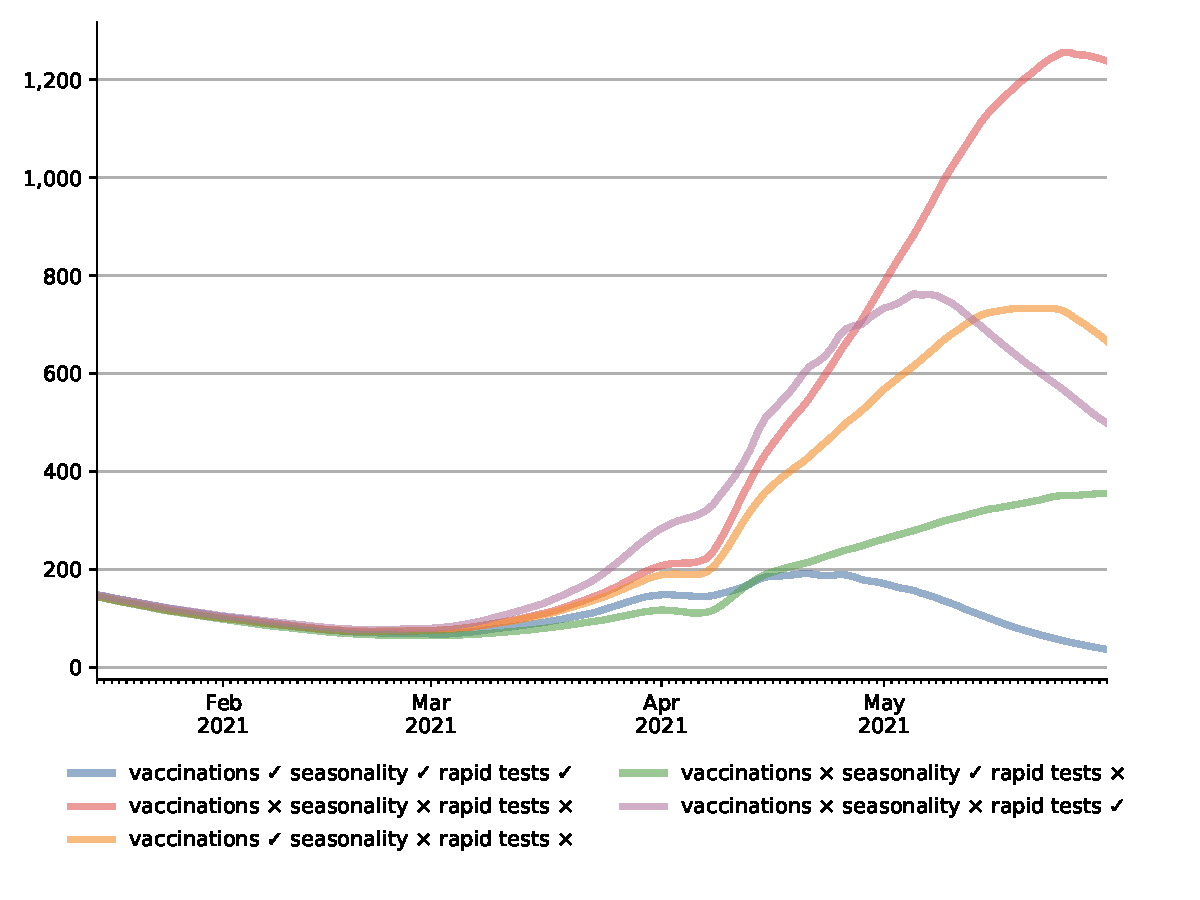
\includegraphics[width=\textwidth]{../figures/results/figures/scenario_comparisons/effect_of_channels_on_pessimistic_scenario/full_new_known_case}
        \caption{{\small Recorded cases: 2021 scenarios}}
        \label{fig:2021_scenarios_recorded}
    \end{subfigure}
    \hfill
    \begin{subfigure}[b]{0.475\textwidth}
        \centering
        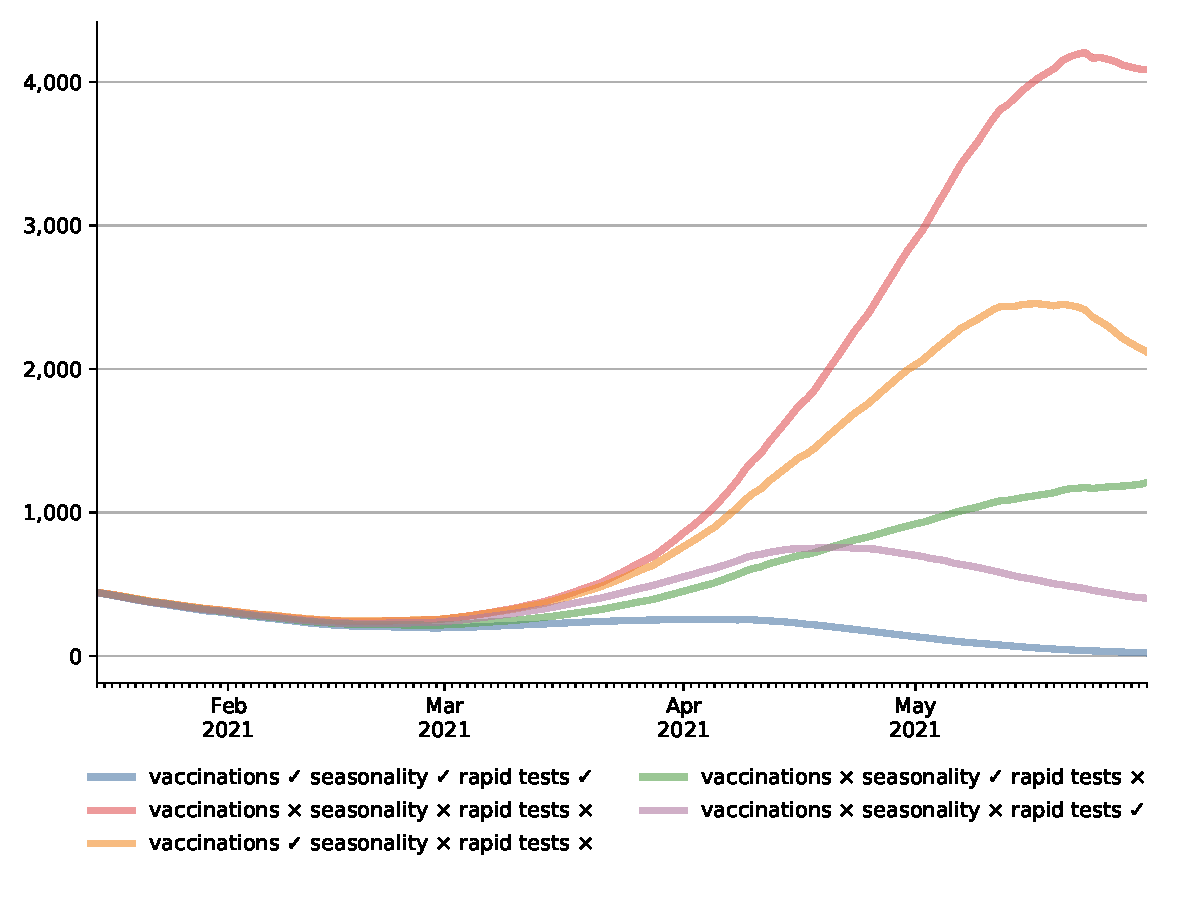
\includegraphics[width=\textwidth]{../figures/results/figures/scenario_comparisons/effect_of_channels_on_pessimistic_scenario/full_newly_infected}
        \caption{{\small Total cases: 2021 scenarios}}
        \label{fig:2021_scenarios_newly_infected}
    \end{subfigure}
    
    \begin{subfigure}[b]{0.475\textwidth}
        \centering
        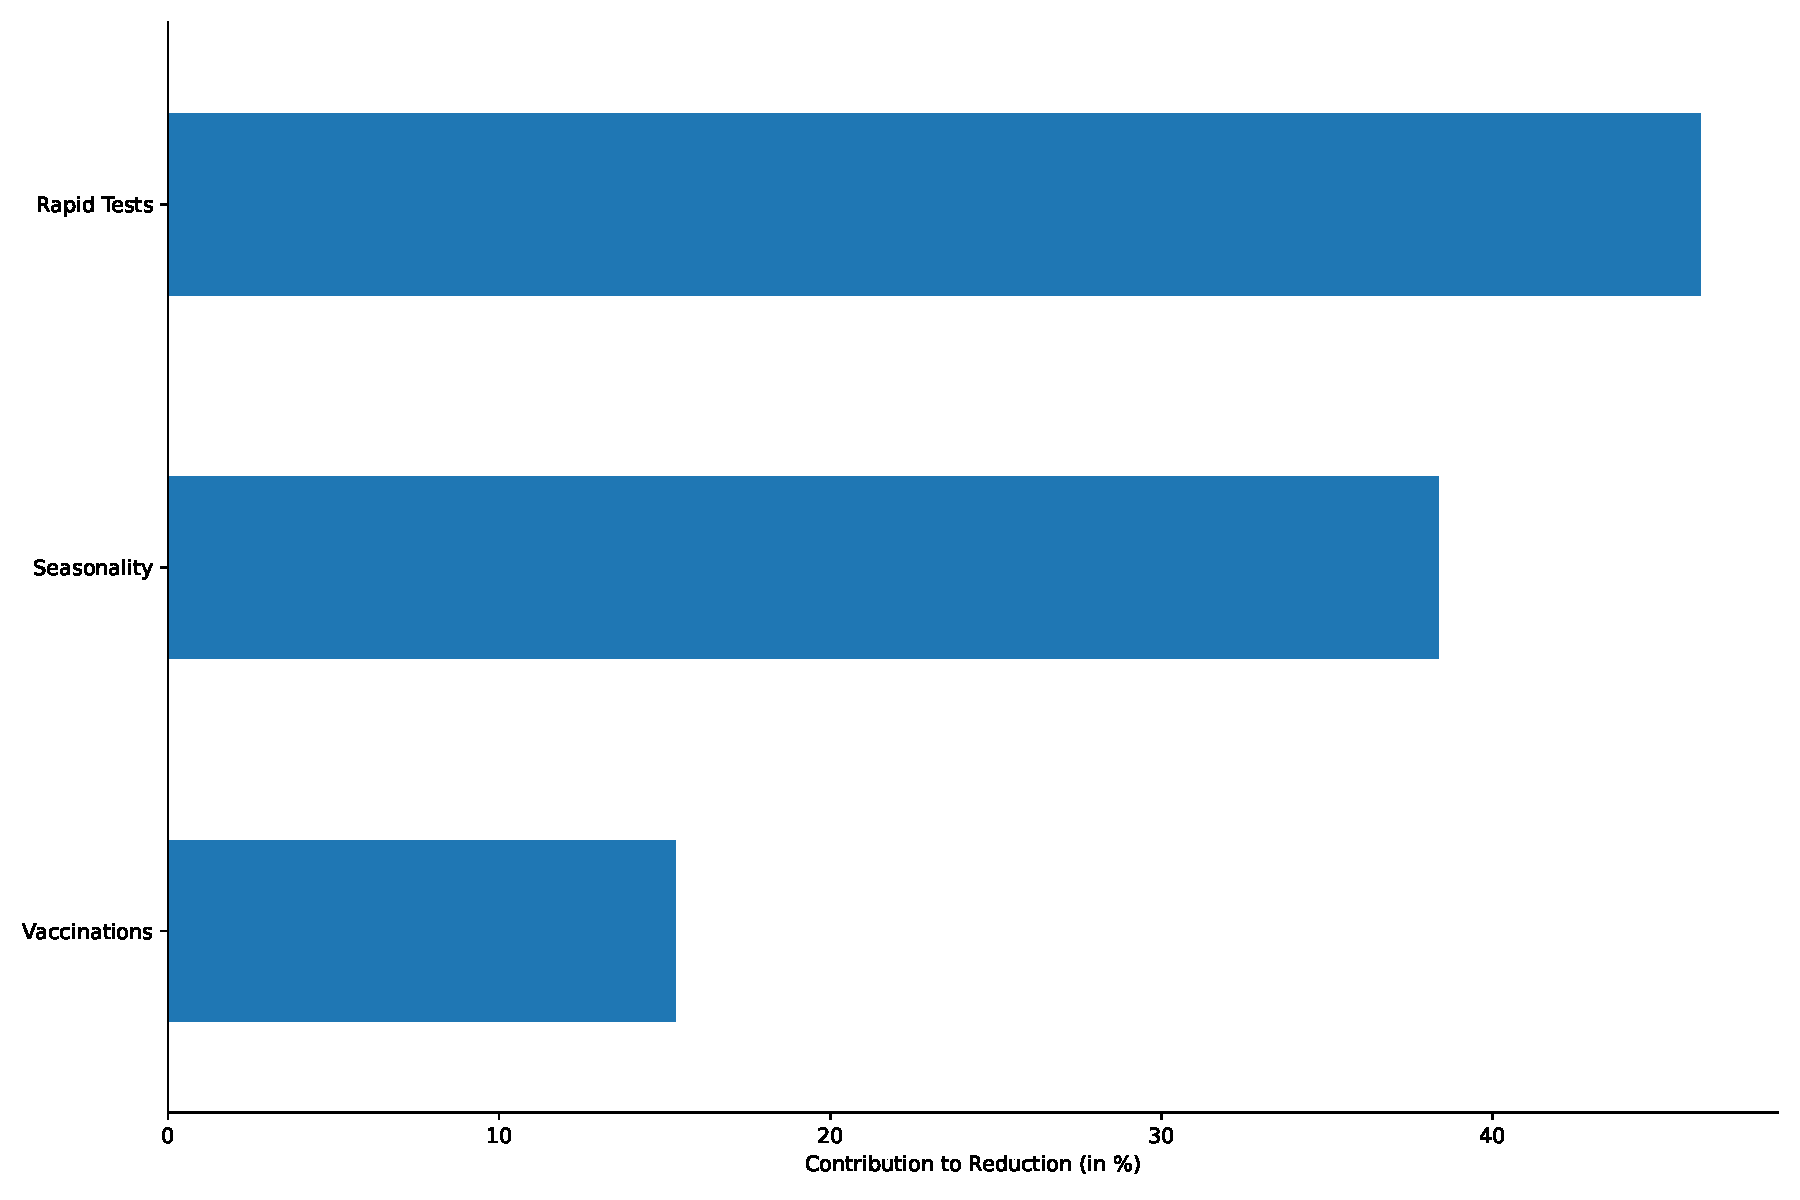
\includegraphics[width=\textwidth]{../figures/full_decomposition}
        
        \vskip2ex
        
        \caption{Decomposition of effects for Figure~\ref{fig:2021_scenarios_newly_infected}.}
        \label{fig:2021_scenarios_decomposition}
    \end{subfigure}
    \hfill
    \begin{subfigure}[b]{0.475\textwidth}
        \centering
        
        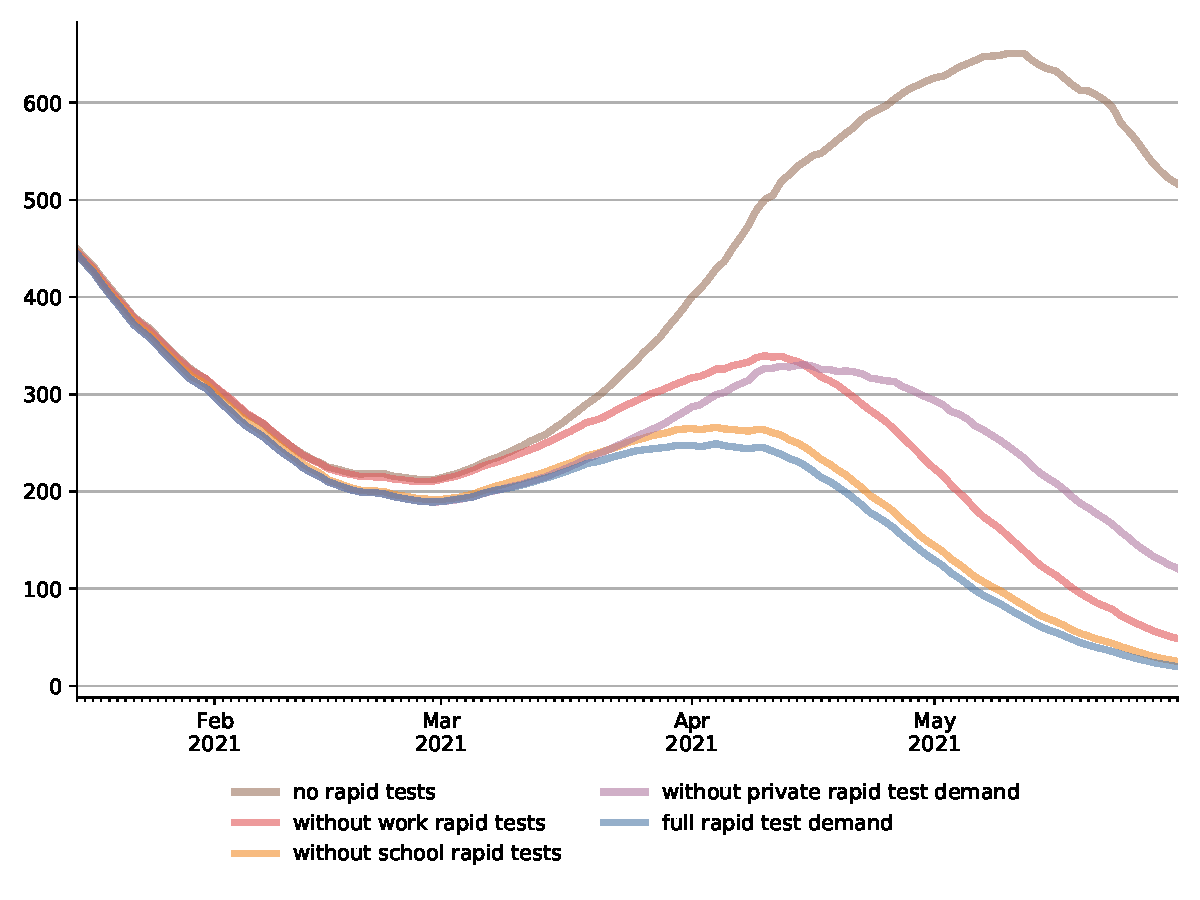
\includegraphics[width=\textwidth]{../figures/results/figures/scenario_comparisons/effect_of_rapid_tests/full_newly_infected}
        \caption{{\small Effects of different types of testing}}
        \label{fig:2021_scenarios_decomposition_tests}
    \end{subfigure}
    
    \caption{The effect of different interventions on recorded and actual infections}
    \label{fig:2021_scenarios_broad}
    
    \floatfoot{\noindent
    Note: All aggregates; See S.XXX for statistics by age group and by geographical region.
    
    The decomposition is based on Shapley values where the individual contribution of a channel is its average contribution over different sizes of coalitions (combinations with other channels). The individual contribution to a coalition is the difference between the effect size of the coalition with the particular channel and without.
    }
\end{figure}

The effect of the vaccination campaign is surprisingly small at first sight. The reasons for this are the slow start---10\% of the population was vaccinated in XX date, 20\% in mid-April\comment[id=HM]{(check!)}---and the focus on older individuals. These groups contribute less to the spread of the disease than others due to a lower number of contacts, see~\ref{fig:assortativity}. It is important to note that the initial focus of the campaign was to prevent deaths and severe disease; the case fatality was rate considerably lower during the third wave when compared to the second (4.4\% between October and February and 1.4\% between March and June).


\clearpage

\section*{writing barrier}

Schooling very contentious. Likely damage to child development.

We show

Screening effect: ...


\begin{figure}[!tp]
    \centering

    \begin{subfigure}[b]{0.475\textwidth}
        \centering
        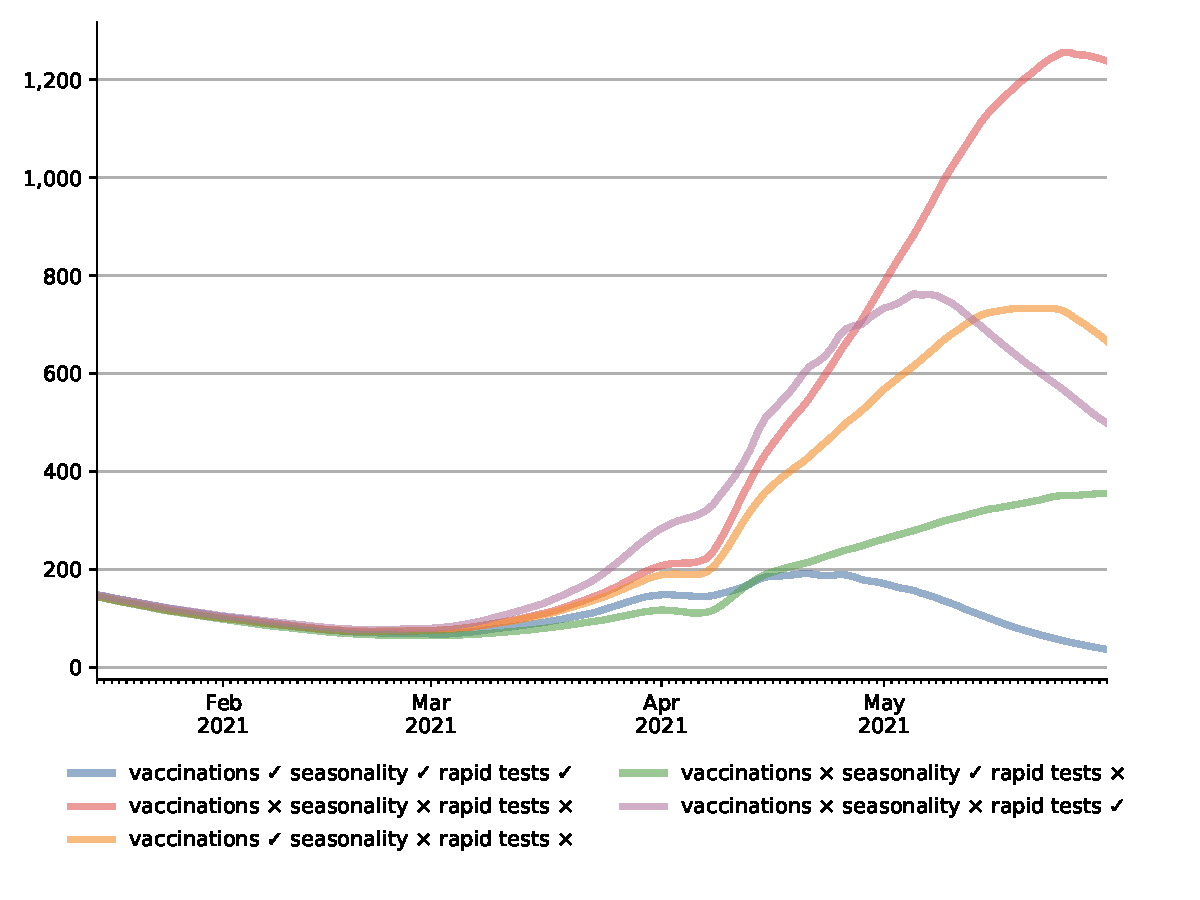
\includegraphics[width=\textwidth]{../figures/results/figures/scenario_comparisons/effect_of_channels_on_pessimistic_scenario/full_new_known_case}
        \caption{{\small Effects of different schooling scenarios after Easter}}
        \label{fig:schooling_scenarios_easter}
    \end{subfigure}
    \hfill
    \begin{subfigure}[b]{0.475\textwidth}
        \centering
        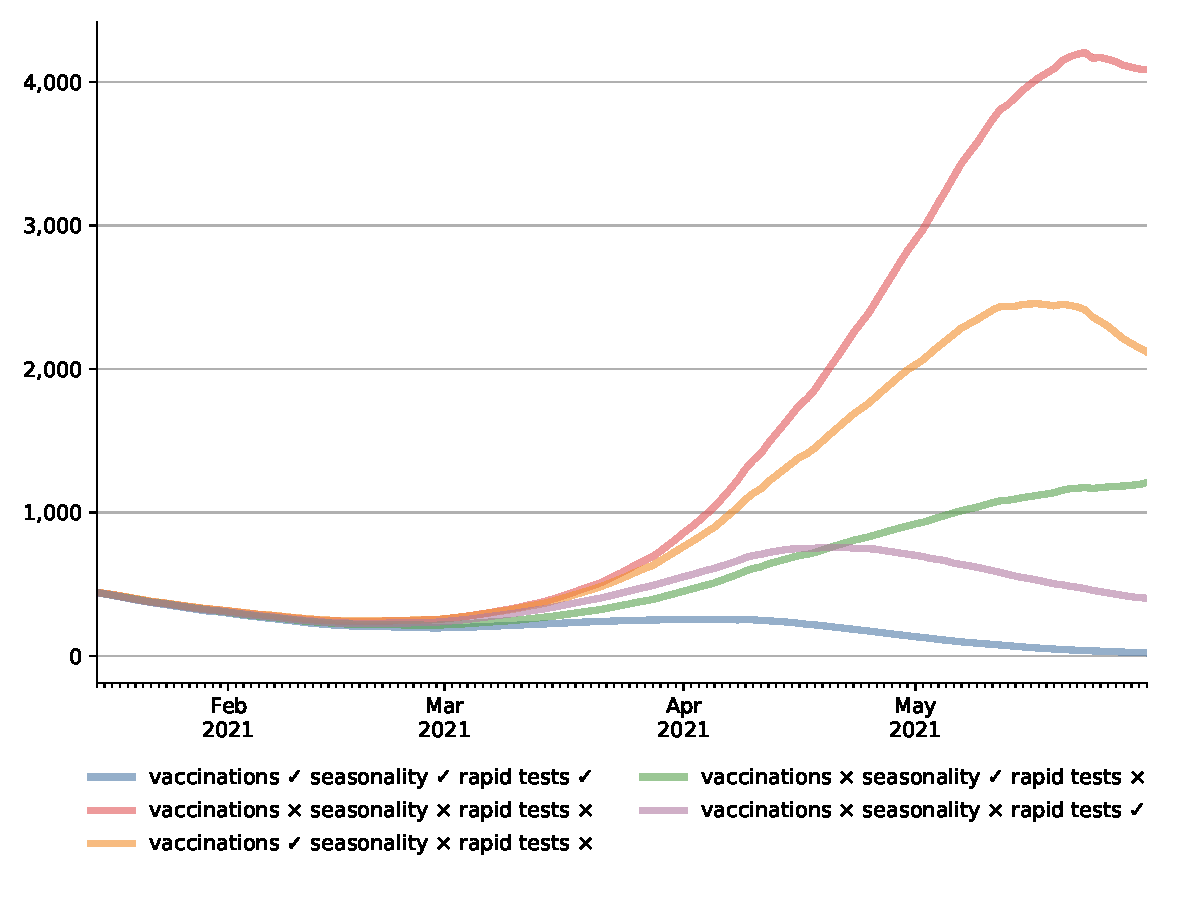
\includegraphics[width=\textwidth]{../figures/results/figures/scenario_comparisons/effect_of_channels_on_pessimistic_scenario/full_newly_infected}
        \caption{{\small TBD}}
        \label{fig:to_be_determined}
    \end{subfigure}
    \vskip3ex

    \caption{Schooling / maybe home office}
    \label{fig:interventions_school}

    \floatfoot{\noindent
        Note: All aggregates; See S.XXX for statistics by age group and by geographical region.
    }

\end{figure}




\paragraph{Points to mention}
\begin{itemize}
    \item If anything too optimistic regarding vaccinations
    \item Social structure / conditional block testing in families important (?)
    \item Trump-effect: More testing = more cases true for how long?
\end{itemize}

% Technical terms should be defined. 

% Symbols, abbreviations, and acronyms should be defined the first time they are used. 

% All tables and figures should be cited in numerical order.

% All data must be shown either in the main text or in the Supplementary Materials or must be available in an established database with accession details provided in the acknowledgements section.

% References to unpublished materials are not allowed to substantiate significant conclusions of the paper.


\section{Supplementary Material}

\begin{enumerate}
    \item Model
    \item Data
    \item Identification and Estimation
\end{enumerate}